\documentclass{scrartcl}\usepackage[]{graphicx}\usepackage[]{color}
%% maxwidth is the original width if it is less than linewidth
%% otherwise use linewidth (to make sure the graphics do not exceed the margin)
\makeatletter
\def\maxwidth{ %
  \ifdim\Gin@nat@width>\linewidth
    \linewidth
  \else
    \Gin@nat@width
  \fi
}
\makeatother

\definecolor{fgcolor}{rgb}{0.345, 0.345, 0.345}
\newcommand{\hlnum}[1]{\textcolor[rgb]{0.686,0.059,0.569}{#1}}%
\newcommand{\hlstr}[1]{\textcolor[rgb]{0.192,0.494,0.8}{#1}}%
\newcommand{\hlcom}[1]{\textcolor[rgb]{0.678,0.584,0.686}{\textit{#1}}}%
\newcommand{\hlopt}[1]{\textcolor[rgb]{0,0,0}{#1}}%
\newcommand{\hlstd}[1]{\textcolor[rgb]{0.345,0.345,0.345}{#1}}%
\newcommand{\hlkwa}[1]{\textcolor[rgb]{0.161,0.373,0.58}{\textbf{#1}}}%
\newcommand{\hlkwb}[1]{\textcolor[rgb]{0.69,0.353,0.396}{#1}}%
\newcommand{\hlkwc}[1]{\textcolor[rgb]{0.333,0.667,0.333}{#1}}%
\newcommand{\hlkwd}[1]{\textcolor[rgb]{0.737,0.353,0.396}{\textbf{#1}}}%

\usepackage{framed}
\makeatletter
\newenvironment{kframe}{%
 \def\at@end@of@kframe{}%
 \ifinner\ifhmode%
  \def\at@end@of@kframe{\end{minipage}}%
  \begin{minipage}{\columnwidth}%
 \fi\fi%
 \def\FrameCommand##1{\hskip\@totalleftmargin \hskip-\fboxsep
 \colorbox{shadecolor}{##1}\hskip-\fboxsep
     % There is no \\@totalrightmargin, so:
     \hskip-\linewidth \hskip-\@totalleftmargin \hskip\columnwidth}%
 \MakeFramed {\advance\hsize-\width
   \@totalleftmargin\z@ \linewidth\hsize
   \@setminipage}}%
 {\par\unskip\endMakeFramed%
 \at@end@of@kframe}
\makeatother

\definecolor{shadecolor}{rgb}{.97, .97, .97}
\definecolor{messagecolor}{rgb}{0, 0, 0}
\definecolor{warningcolor}{rgb}{1, 0, 1}
\definecolor{errorcolor}{rgb}{1, 0, 0}
\newenvironment{knitrout}{}{} % an empty environment to be redefined in TeX

\usepackage{alltt}
\usepackage[utf8]{inputenc}
\usepackage{graphicx}%GRaphiken
\usepackage{tabularx}%Tabellen!
\usepackage[english]{babel}% Zeilentrennung besser
\usepackage{url}% Urls besser
\usepackage{textcomp}% Sonderzeichen
\usepackage{amsmath}%maths / equations
\usepackage{helvet}% Schrift Helvetica
% \usepackage[helvet]{sfmath}% Helvet also in Math modes
% \renewcommand\familydefault{\sfdefault}
\usepackage{sansmath} % sans in math
\usepackage{todonotes}
\usepackage[
	left=3cm,
	right=2cm,
	top=1.5cm,
	bottom=1cm
	,
	includeheadfoot
	]{geometry}														% Satzspiegel
\usepackage[
	round,	%(defaultage in the main file and \input ) for round parentheses;
	%square,	% for square brackets;
	%curly,	% for curly braces;
	%angle,	% for angle brackets;
	colon,	% (default) to separate multiple citations with colons;
	%comma,	% to use commas as separaters;
	authoryear,% (default) for author-year citations;
	%numbers,	% for numerical citations;
	%super,	% for superscripted numerical citations, as in Nature;
	sort,		% orders multiple citations into the sequence in which they appear in the list of 				references;
	%sort&compress,    % as sort but in addition multiple numerical citations
                   % are compressed if possible (as 3-6, 15);
	%longnamesfirst,  % makes the first citation of any reference the equivalent of
                   % the starred variant (full author list) and subsequent citations
                   %normal (abbreviated list);
	%sectionbib,      % redefines \thebibliography to issue \section* instead of \chapter*;
                   % valid only for classes with a \chapter command;
                   % to be used with the chapterbib package;
	%nonamebreak,     % keeps all the authors names in a citation on one line;
                   %causes overfull hboxes but helps with some hyperref problems.
]{natbib}											    			% Literaturverzeichnis
\usepackage{scrhack}   % kills \float@addtolists!  warning
\usepackage[pdfpagelabels,plainpages=false, pageanchor=false]{hyperref}	


%% andere Einstellungen
\linespread{1}% 1.5 Zeilenabstand			
\graphicspath{{fig/}}                     % path to graphics

%% ----------------------------------------------------------------------------
\title{Ecotoxicology is not normal.}
\subtitle{A comparison of statistical approaches for analysis of count and proportion data in ecotoxicology.}
\author{Eduard Szöcs, Ralf B. Schäfer}
\date{\today}


% ----------------------------------------------------------------------------
\IfFileExists{upquote.sty}{\usepackage{upquote}}{}
\begin{document}
\maketitle

\setcounter{section}{1}
\section{Supplement 2 - R examples}
\subsection{Count data example}
\subsubsection{Introduction}
In this example we will analyse data from \citep{brock_minimum_2015}.
The data are count of mayfly larvae in Macroinvertebrate Artificial Substrate Samplers in 18 mesocosms at one sampling day.
There are 5 treatments and one control group.

First we load the data and bring it to the long format and remove NA values.
\begin{knitrout}
\definecolor{shadecolor}{rgb}{0.969, 0.969, 0.969}\color{fgcolor}\begin{kframe}
\begin{alltt}
\hlstd{df} \hlkwb{<-} \hlkwd{read.table}\hlstd{(}\hlkwc{header} \hlstd{=} \hlnum{TRUE}\hlstd{,} \hlkwc{text} \hlstd{=} \hlstr{'Control  T0.1 T0.3  T1  T3  T10
175 29  27  36  26  20
65  114 78  11  13  37
154 72  27  105 33  NA
83  NA  NA  NA  NA  NA
'}\hlstd{)}
\hlkwd{require}\hlstd{(reshape2)}
\hlstd{dfm} \hlkwb{<-} \hlkwd{melt}\hlstd{(df,} \hlkwc{value.name} \hlstd{=} \hlstr{'abu'}\hlstd{,} \hlkwc{variable.name} \hlstd{=} \hlstr{'treatment'}\hlstd{)}
\hlstd{dfm} \hlkwb{<-} \hlstd{dfm[}\hlopt{!}\hlkwd{is.na}\hlstd{(dfm[}\hlstr{'abu'}\hlstd{]), ]}
\hlkwd{head}\hlstd{(dfm)}
\end{alltt}
\begin{verbatim}
##   treatment abu
## 1   Control 175
## 2   Control  65
## 3   Control 154
## 4   Control  83
## 5      T0.1  29
## 6      T0.1 114
\end{verbatim}
\end{kframe}
\end{knitrout}
This give a table with two columns - one indicating the treatment and one with the measured abundances.

  
Let's have a first look at the data:
\begin{knitrout}
\definecolor{shadecolor}{rgb}{0.969, 0.969, 0.969}\color{fgcolor}\begin{kframe}
\begin{alltt}
\hlkwd{boxplot}\hlstd{(abu} \hlopt{~} \hlstd{treatment,} \hlkwc{data} \hlstd{= dfm,} \hlkwc{xlab} \hlstd{=} \hlstr{'Treatment'}\hlstd{,}
        \hlkwc{ylab} \hlstd{=} \hlstr{'Count'}\hlstd{,} \hlkwc{col} \hlstd{=} \hlstr{'grey75'}\hlstd{,} \hlkwc{main} \hlstd{=} \hlstr{'Raw abundances'}\hlstd{)}
\end{alltt}
\end{kframe}
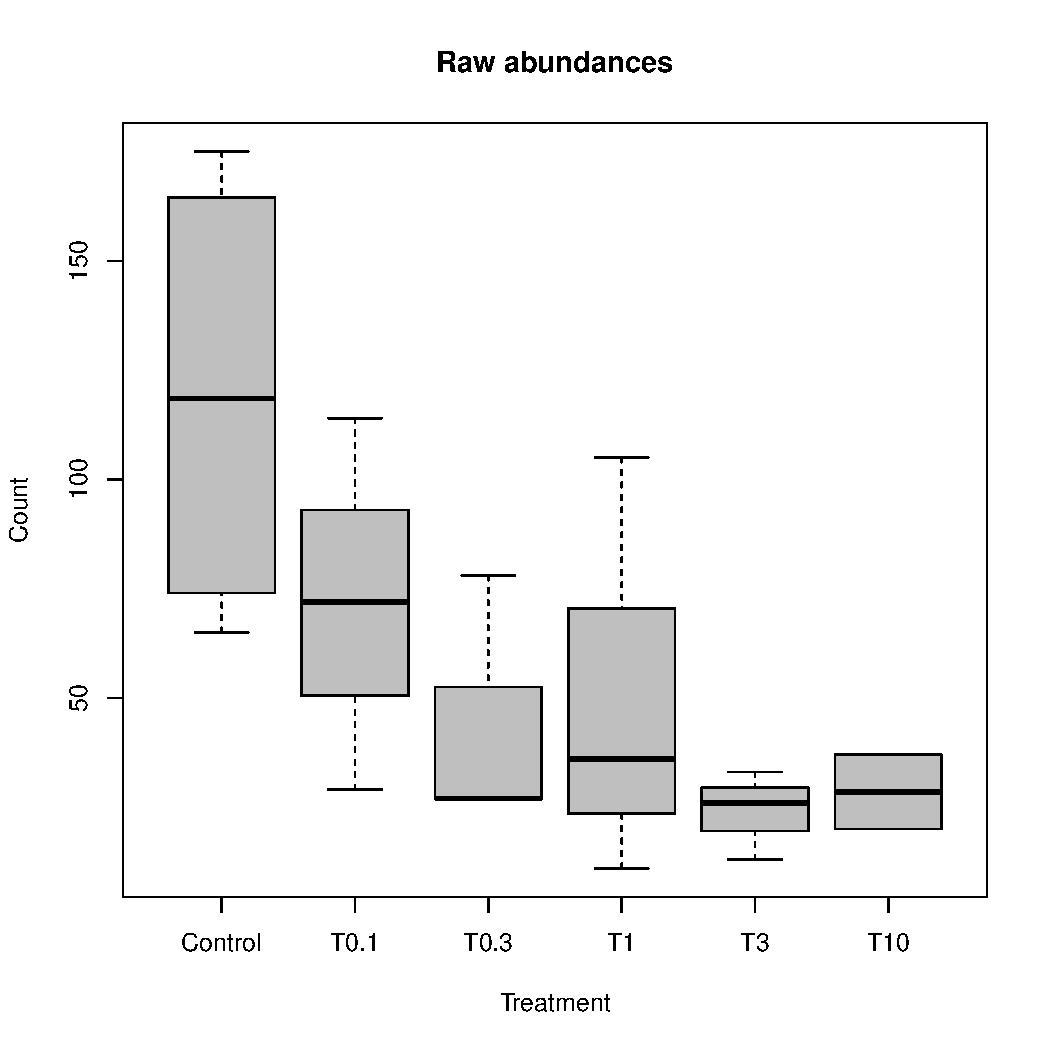
\includegraphics[width=0.5\textwidth]{figure/count_raw_plot-1} 

\end{knitrout}
We clearly see a treatment related response. 
Moreover, we may note that variances are increasing with increasing abundances.

\subsubsection{Transforming data}
Next we transform the data using a ln(Ax + 1) transformation.
A is chosen so that the term Ax equals two for the lowest non-zero abundance.
We add these transformed abundances as column to our table.

\begin{knitrout}
\definecolor{shadecolor}{rgb}{0.969, 0.969, 0.969}\color{fgcolor}\begin{kframe}
\begin{alltt}
\hlstd{A} \hlkwb{<-} \hlnum{2} \hlopt{/} \hlkwd{min}\hlstd{(dfm}\hlopt{$}\hlstd{abu[dfm}\hlopt{$}\hlstd{abu} \hlopt{!=} \hlnum{0}\hlstd{])}
\hlstd{A}
\end{alltt}
\begin{verbatim}
## [1] 0.1818182
\end{verbatim}
\begin{alltt}
\hlstd{dfm}\hlopt{$}\hlstd{abu_t} \hlkwb{<-} \hlkwd{log}\hlstd{(A} \hlopt{*} \hlstd{dfm}\hlopt{$}\hlstd{abu} \hlopt{+} \hlnum{1}\hlstd{)}
\end{alltt}
\end{kframe}
\end{knitrout}


It looks like the transformation does a good job in equalizing the variances:
\begin{knitrout}
\definecolor{shadecolor}{rgb}{0.969, 0.969, 0.969}\color{fgcolor}\begin{kframe}
\begin{alltt}
\hlkwd{boxplot}\hlstd{(abu_t} \hlopt{~} \hlstd{treatment,} \hlkwc{data} \hlstd{= dfm,}
        \hlkwc{xlab} \hlstd{=} \hlstr{'Treatment'}\hlstd{,} \hlkwc{ylab} \hlstd{=} \hlstr{'Transf. Counts'}\hlstd{,}
        \hlkwc{col} \hlstd{=} \hlstr{'grey75'}\hlstd{,} \hlkwc{main} \hlstd{=} \hlstr{'Transformed abundances'}\hlstd{)}
\end{alltt}
\end{kframe}
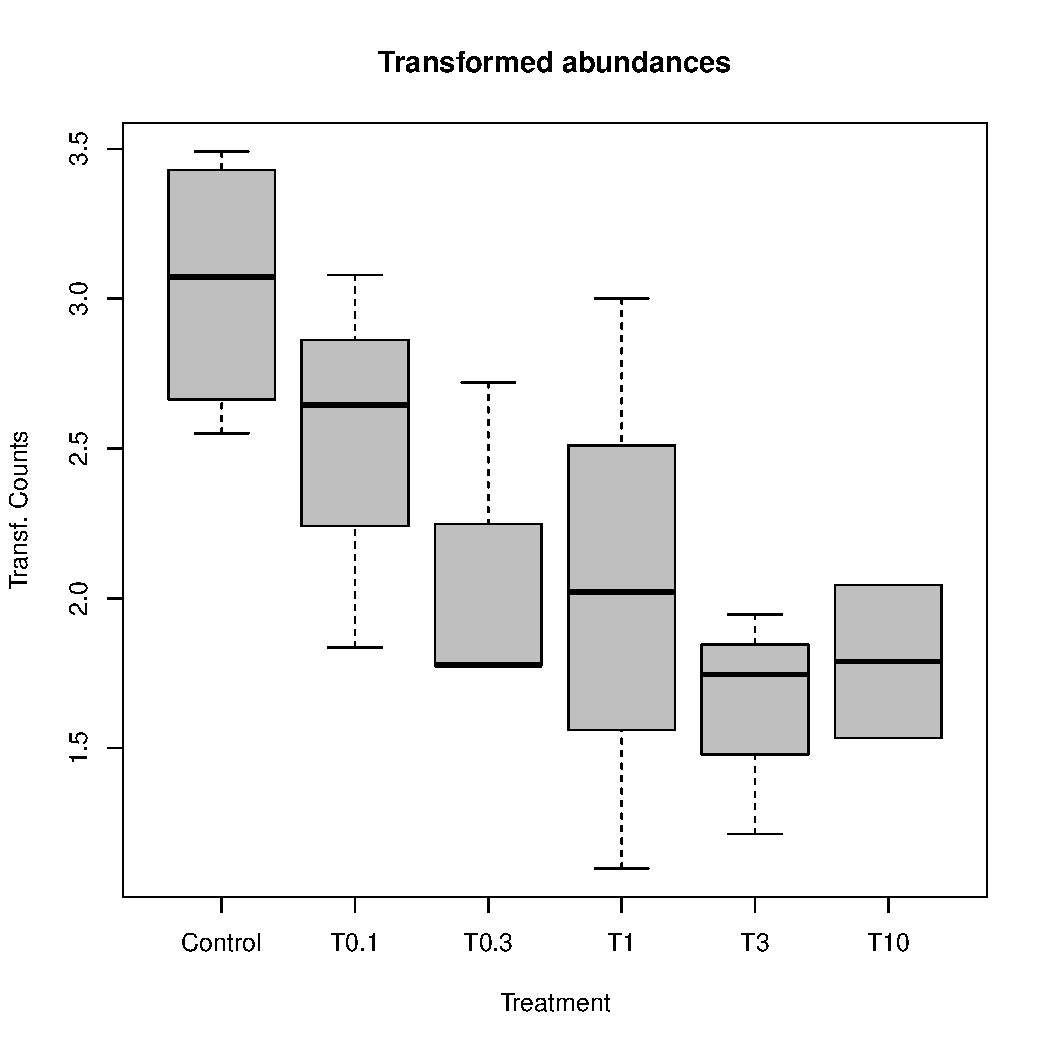
\includegraphics[width=0.5\textwidth]{figure/plot_count_trans-1} 

\end{knitrout}


\subsubsection{Assuming a normal distribution of transformed abundances}
We start with analysing this data assuming a normal distribution of the transformed abundances with constant variance.
This can be easily done using the \texttt{lm()} function:

\begin{knitrout}
\definecolor{shadecolor}{rgb}{0.969, 0.969, 0.969}\color{fgcolor}\begin{kframe}
\begin{alltt}
\hlstd{modlm} \hlkwb{<-} \hlkwd{lm}\hlstd{(abu_t} \hlopt{~} \hlstd{treatment,} \hlkwc{data} \hlstd{= dfm)}
\end{alltt}
\end{kframe}
\end{knitrout}

The \texttt{summary()} gives the estimated parameters with standard errors and Wald t tests:
\begin{knitrout}
\definecolor{shadecolor}{rgb}{0.969, 0.969, 0.969}\color{fgcolor}\begin{kframe}
\begin{alltt}
\hlkwd{summary}\hlstd{(modlm)}
\end{alltt}
\begin{verbatim}
## 
## Call:
## lm(formula = abu_t ~ treatment, data = dfm)
## 
## Residuals:
##      Min       1Q   Median       3Q      Max 
## -0.94133 -0.31454  0.04576  0.31813  0.96033 
## 
## Coefficients:
##               Estimate Std. Error t value Pr(>|t|)    
## (Intercept)     3.0468     0.2970  10.260 2.71e-07 ***
## treatmentT0.1  -0.5267     0.4536  -1.161  0.26814    
## treatmentT0.3  -0.9558     0.4536  -2.107  0.05682 .  
## treatmentT1    -1.0069     0.4536  -2.220  0.04646 *  
## treatmentT3    -1.4121     0.4536  -3.113  0.00897 ** 
## treatmentT10   -1.2575     0.5144  -2.445  0.03089 *  
## ---
## Signif. codes:  0 '***' 0.001 '**' 0.01 '*' 0.05 '.' 0.1 ' ' 1
## 
## Residual standard error: 0.5939 on 12 degrees of freedom
## Multiple R-squared:  0.5167,	Adjusted R-squared:  0.3154 
## F-statistic: 2.566 on 5 and 12 DF,  p-value: 0.08406
\end{verbatim}
\end{kframe}
\end{knitrout}

Or, if you want to have the ANOVA table with an F-test:
\begin{knitrout}
\definecolor{shadecolor}{rgb}{0.969, 0.969, 0.969}\color{fgcolor}\begin{kframe}
\begin{alltt}
\hlkwd{summary.aov}\hlstd{(modlm)}
\end{alltt}
\begin{verbatim}
##             Df Sum Sq Mean Sq F value Pr(>F)  
## treatment    5  4.526  0.9052   2.566 0.0841 .
## Residuals   12  4.233  0.3528                 
## ---
## Signif. codes:  0 '***' 0.001 '**' 0.01 '*' 0.05 '.' 0.1 ' ' 1
\end{verbatim}
\end{kframe}
\end{knitrout}

From this output we might infer that we cannot detect any treatment effect (F = 2.566, p = 0.084).
Let's move on to the LOEC determination. This can be easily done using the multcomp package \citep{hothorn_simultaneous_2008}:
Here we perform a one-sided (\texttt{alternative='less'}) Dunnett (\texttt{mcp(treatment='Dunnett')}) test.
\begin{knitrout}
\definecolor{shadecolor}{rgb}{0.969, 0.969, 0.969}\color{fgcolor}\begin{kframe}
\begin{alltt}
\hlkwd{require}\hlstd{(multcomp)}
\hlcom{# one-sided Dunnett test}
\hlkwd{summary}\hlstd{(}\hlkwd{glht}\hlstd{(modlm,} \hlkwc{linfct} \hlstd{=} \hlkwd{mcp}\hlstd{(}\hlkwc{treatment} \hlstd{=} \hlstr{'Dunnett'}\hlstd{),}  \hlkwc{alternative} \hlstd{=} \hlstr{'less'}\hlstd{))}
\end{alltt}
\begin{verbatim}
## 
## 	 Simultaneous Tests for General Linear Hypotheses
## 
## Multiple Comparisons of Means: Dunnett Contrasts
## 
## 
## Fit: lm(formula = abu_t ~ treatment, data = dfm)
## 
## Linear Hypotheses:
##                     Estimate Std. Error t value Pr(<t)  
## T0.1 - Control >= 0  -0.5267     0.4536  -1.161 0.3841  
## T0.3 - Control >= 0  -0.9558     0.4536  -2.107 0.1030  
## T1 - Control >= 0    -1.0069     0.4536  -2.220 0.0859 .
## T3 - Control >= 0    -1.4121     0.4536  -3.113 0.0182 *
## T10 - Control >= 0   -1.2575     0.5144  -2.445 0.0588 .
## ---
## Signif. codes:  0 '***' 0.001 '**' 0.01 '*' 0.05 '.' 0.1 ' ' 1
## (Adjusted p values reported -- single-step method)
\end{verbatim}
\end{kframe}
\end{knitrout}

This indicates that only treatment 3 shows a statistically significant from control and is the determined LOEC.




\subsubsection{Assuming a Poisson distribution of abundances}

Instead transforming the data, we could assume a Poisson distribution and fit a GLM to this data.
This can be done using the \texttt{glm()} function:
\begin{knitrout}
\definecolor{shadecolor}{rgb}{0.969, 0.969, 0.969}\color{fgcolor}\begin{kframe}
\begin{alltt}
\hlstd{modpois} \hlkwb{<-} \hlkwd{glm}\hlstd{(abu} \hlopt{~} \hlstd{treatment,} \hlkwc{data} \hlstd{= dfm,} \hlkwc{family} \hlstd{=} \hlkwd{poisson}\hlstd{(}\hlkwc{link} \hlstd{=} \hlstr{'log'}\hlstd{))}
\end{alltt}
\end{kframe}
\end{knitrout}

, \texttt{family = poisson(link = 'log')} specifies that we want to fit a poisson model using a log link between response and predictors.

The \texttt{summary} gives the estimated parameters, standard errors and Wald Z tests:
\begin{knitrout}
\definecolor{shadecolor}{rgb}{0.969, 0.969, 0.969}\color{fgcolor}\begin{kframe}
\begin{alltt}
\hlkwd{summary}\hlstd{(modpois)}
\end{alltt}
\begin{verbatim}
## 
## Call:
## glm(formula = abu ~ treatment, family = poisson(link = "log"), 
##     data = dfm)
## 
## Deviance Residuals: 
##     Min       1Q   Median       3Q      Max  
## -6.7625  -2.7621  -0.8219   2.7172   6.6602  
## 
## Coefficients:
##               Estimate Std. Error z value Pr(>|z|)    
## (Intercept)    4.78122    0.04579 104.423  < 2e-16 ***
## treatmentT0.1 -0.50920    0.08214  -6.199 5.69e-10 ***
## treatmentT0.3 -0.99703    0.09835 -10.138  < 2e-16 ***
## treatmentT1   -0.85595    0.09314  -9.190  < 2e-16 ***
## treatmentT3   -1.60317    0.12643 -12.680  < 2e-16 ***
## treatmentT10  -1.43132    0.14014 -10.213  < 2e-16 ***
## ---
## Signif. codes:  0 '***' 0.001 '**' 0.01 '*' 0.05 '.' 0.1 ' ' 1
## 
## (Dispersion parameter for poisson family taken to be 1)
## 
##     Null deviance: 604.79  on 17  degrees of freedom
## Residual deviance: 273.77  on 12  degrees of freedom
## AIC: 387.63
## 
## Number of Fisher Scoring iterations: 5
\end{verbatim}
\end{kframe}
\end{knitrout}

To perform a LR-Test we can used \texttt{drop1()}:
\begin{knitrout}
\definecolor{shadecolor}{rgb}{0.969, 0.969, 0.969}\color{fgcolor}\begin{kframe}
\begin{alltt}
\hlkwd{drop1}\hlstd{(modpois,} \hlkwc{test} \hlstd{=} \hlstr{'Chisq'}\hlstd{)}
\end{alltt}
\begin{verbatim}
## Single term deletions
## 
## Model:
## abu ~ treatment
##           Df Deviance    AIC    LRT  Pr(>Chi)    
## <none>         273.77 387.63                     
## treatment  5   604.79 708.64 331.02 < 2.2e-16 ***
## ---
## Signif. codes:  0 '***' 0.001 '**' 0.01 '*' 0.05 '.' 0.1 ' ' 1
\end{verbatim}
\end{kframe}
\end{knitrout}
which indicates a strong treatment effect.

But is a poisson distribution appropriate here? 
A property of the poisson distribution is that its variance is equal to the mean. 
A simple diagnostic would be to plot group variances vs. group means:

\begin{knitrout}
\definecolor{shadecolor}{rgb}{0.969, 0.969, 0.969}\color{fgcolor}\begin{kframe}
\begin{alltt}
\hlkwd{require}\hlstd{(plyr)}
\hlcom{# mean and variance per treatment}
\hlstd{musd} \hlkwb{<-} \hlkwd{ddply}\hlstd{(dfm,} \hlkwd{.}\hlstd{(treatment), summarise,}
              \hlkwc{mu} \hlstd{=} \hlkwd{mean}\hlstd{(abu),}
              \hlkwc{var} \hlstd{=} \hlkwd{var}\hlstd{(abu))}
\hlstd{musd}
\end{alltt}
\begin{verbatim}
##   treatment        mu      var
## 1   Control 119.25000 2857.583
## 2      T0.1  71.66667 1806.333
## 3      T0.3  44.00000  867.000
## 4        T1  50.66667 2370.333
## 5        T3  24.00000  103.000
## 6       T10  28.50000  144.500
\end{verbatim}
\begin{alltt}
\hlcom{# plot}
\hlkwd{plot}\hlstd{(var} \hlopt{~} \hlstd{mu,} \hlkwc{data} \hlstd{= musd,} \hlkwc{xlab} \hlstd{=} \hlstr{'mean'}\hlstd{,} \hlkwc{ylab} \hlstd{=} \hlstr{'variance'}\hlstd{,} \hlkwc{main} \hlstd{=} \hlstr{'Mean-variance relationships'}\hlstd{)}
\hlcom{# poisson}
\hlkwd{abline}\hlstd{(}\hlkwc{a} \hlstd{=} \hlnum{0}\hlstd{,} \hlkwc{b} \hlstd{=} \hlnum{1}\hlstd{,} \hlkwc{col} \hlstd{=} \hlstr{'darkblue'}\hlstd{,} \hlkwc{lwd} \hlstd{=} \hlnum{2}\hlstd{)}
\hlcom{# quasi-Poisson}
\hlkwd{abline}\hlstd{(}\hlkwc{a} \hlstd{=} \hlnum{0}\hlstd{,} \hlkwc{b} \hlstd{=} \hlnum{22.41}\hlstd{,} \hlkwc{col} \hlstd{=} \hlstr{'darkgreen'}\hlstd{,} \hlkwc{lwd} \hlstd{=} \hlnum{2}\hlstd{)}
\hlcom{# Negative binomial}
\hlkwd{curve}\hlstd{(x} \hlopt{+} \hlstd{(x}\hlopt{^}\hlnum{2} \hlopt{/} \hlnum{3.91}\hlstd{),} \hlkwc{from} \hlstd{=} \hlnum{24}\hlstd{,} \hlkwc{to} \hlstd{=} \hlnum{119.25}\hlstd{,} \hlkwc{add} \hlstd{=} \hlnum{TRUE}\hlstd{,} \hlkwc{col} \hlstd{=} \hlstr{'darkred'}\hlstd{,} \hlkwc{lwd} \hlstd{=} \hlnum{2}\hlstd{)}
\hlkwd{legend}\hlstd{(}\hlstr{'topleft'}\hlstd{,} \hlkwd{c}\hlstd{(}\hlstr{'NB(k = 3.91)'}\hlstd{,} \hlstr{'Poisson'}\hlstd{,} \hlstr{'Quasi-Poisson(t = 22.4)'}\hlstd{),}
       \hlkwc{col} \hlstd{=} \hlkwd{c}\hlstd{(}\hlstr{'darkred'}\hlstd{,} \hlstr{'darkblue'}\hlstd{,} \hlstr{'darkgreen'}\hlstd{),}
       \hlkwc{lty} \hlstd{=} \hlkwd{c}\hlstd{(}\hlnum{1}\hlstd{,}\hlnum{1}\hlstd{,} \hlnum{1}\hlstd{),}
       \hlkwc{lwd} \hlstd{=} \hlkwd{c}\hlstd{(}\hlnum{2}\hlstd{,}\hlnum{2}\hlstd{,} \hlnum{2}\hlstd{))}
\end{alltt}
\end{kframe}
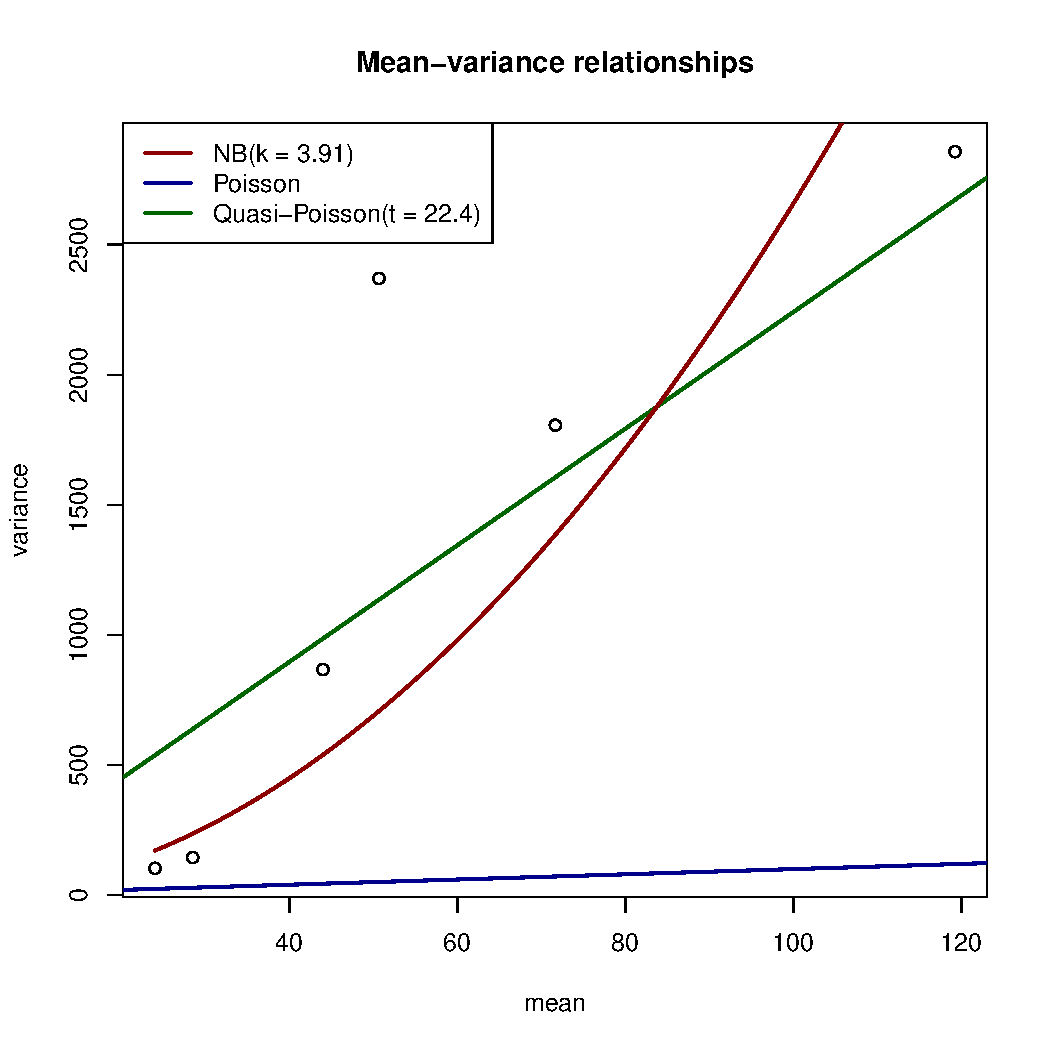
\includegraphics[width=0.5\textwidth]{figure/mod_count_meanvar-1} 

\end{knitrout}

I also added the assumed mean-variance relationships of the Poisson, quasi-Poisson and negative binomial models.
We clearly see that the variance increases much more than would be expected under the poisson distribution (the data is overdispersed).
Moreover, we could check overdispersion from the \texttt{summary}:
If the ratio of residual deviance to degrees of freedom is \textgreater 1 the data is overdispersed.


\subsubsection{Assuming a quasi-Poisson distribution of abundances}
The plot suggests that the variance may increasing stronger then the mean and quasi-Poisson or negative binomial models might be more appropriate for this data.
Fitting a quasi-Poisson GLM is straight forward:
\begin{knitrout}
\definecolor{shadecolor}{rgb}{0.969, 0.969, 0.969}\color{fgcolor}\begin{kframe}
\begin{alltt}
\hlstd{modqpois} \hlkwb{<-} \hlkwd{glm}\hlstd{(abu} \hlopt{~} \hlstd{treatment,} \hlkwc{data} \hlstd{= dfm,} \hlkwc{family} \hlstd{= quasipoisson)}
\end{alltt}
\end{kframe}
\end{knitrout}

The summary gives the estimated parameters:
\begin{knitrout}
\definecolor{shadecolor}{rgb}{0.969, 0.969, 0.969}\color{fgcolor}\begin{kframe}
\begin{alltt}
\hlkwd{summary}\hlstd{(modqpois)}
\end{alltt}
\begin{verbatim}
## 
## Call:
## glm(formula = abu ~ treatment, family = quasipoisson, data = dfm)
## 
## Deviance Residuals: 
##     Min       1Q   Median       3Q      Max  
## -6.7625  -2.7621  -0.8219   2.7172   6.6602  
## 
## Coefficients:
##               Estimate Std. Error t value Pr(>|t|)    
## (Intercept)     4.7812     0.2168  22.058 4.43e-11 ***
## treatmentT0.1  -0.5092     0.3889  -1.309   0.2149    
## treatmentT0.3  -0.9970     0.4656  -2.142   0.0534 .  
## treatmentT1    -0.8560     0.4409  -1.941   0.0761 .  
## treatmentT3    -1.6032     0.5985  -2.679   0.0201 *  
## treatmentT10   -1.4313     0.6634  -2.157   0.0519 .  
## ---
## Signif. codes:  0 '***' 0.001 '**' 0.01 '*' 0.05 '.' 0.1 ' ' 1
## 
## (Dispersion parameter for quasipoisson family taken to be 22.41055)
## 
##     Null deviance: 604.79  on 17  degrees of freedom
## Residual deviance: 273.77  on 12  degrees of freedom
## AIC: NA
## 
## Number of Fisher Scoring iterations: 5
\end{verbatim}
\end{kframe}
\end{knitrout}

with the dispersion parameter $\Theta = 22.41055$. 
Note, that the parameter estimates are the same as from the Poisson model, only the standard errors are scaled/wider.

An F-test can be performed using \texttt{drop1()}:
\begin{knitrout}
\definecolor{shadecolor}{rgb}{0.969, 0.969, 0.969}\color{fgcolor}\begin{kframe}
\begin{alltt}
\hlkwd{drop1}\hlstd{(modqpois,} \hlkwc{test} \hlstd{=} \hlstr{'F'}\hlstd{)}
\end{alltt}
\begin{verbatim}
## Single term deletions
## 
## Model:
## abu ~ treatment
##           Df Deviance F value  Pr(>F)  
## <none>         273.77                  
## treatment  5   604.79  2.9019 0.06059 .
## ---
## Signif. codes:  0 '***' 0.001 '**' 0.01 '*' 0.05 '.' 0.1 ' ' 1
\end{verbatim}
\end{kframe}
\end{knitrout}
, which also indicates no treatment effect.

The LOEC can be determined with \texttt{multcomp}:
\begin{knitrout}
\definecolor{shadecolor}{rgb}{0.969, 0.969, 0.969}\color{fgcolor}\begin{kframe}
\begin{alltt}
\hlkwd{summary}\hlstd{(}\hlkwd{glht}\hlstd{(modqpois,} \hlkwc{linfct} \hlstd{=} \hlkwd{mcp}\hlstd{(}\hlkwc{treatment} \hlstd{=} \hlstr{'Dunnett'}\hlstd{),}  \hlkwc{alternative} \hlstd{=} \hlstr{'less'}\hlstd{))}
\end{alltt}
\begin{verbatim}
## 
## 	 Simultaneous Tests for General Linear Hypotheses
## 
## Multiple Comparisons of Means: Dunnett Contrasts
## 
## 
## Fit: glm(formula = abu ~ treatment, family = quasipoisson, data = dfm)
## 
## Linear Hypotheses:
##                     Estimate Std. Error z value Pr(<z)  
## T0.1 - Control >= 0  -0.5092     0.3889  -1.309 0.3515  
## T0.3 - Control >= 0  -0.9970     0.4656  -2.142 0.0737 .
## T1 - Control >= 0    -0.8560     0.4409  -1.941 0.1154  
## T3 - Control >= 0    -1.6032     0.5985  -2.679 0.0179 *
## T10 - Control >= 0   -1.4313     0.6634  -2.157 0.0710 .
## ---
## Signif. codes:  0 '***' 0.001 '**' 0.01 '*' 0.05 '.' 0.1 ' ' 1
## (Adjusted p values reported -- single-step method)
\end{verbatim}
\end{kframe}
\end{knitrout}



\subsubsection{Assuming a negative binomial distribution of abundances}
To fit a negative binomial GLM we could use \texttt{glm.nb()} from the MASS package \citep{venables_modern_2002}:
\begin{knitrout}
\definecolor{shadecolor}{rgb}{0.969, 0.969, 0.969}\color{fgcolor}\begin{kframe}
\begin{alltt}
\hlkwd{require}\hlstd{(MASS)}
\hlstd{modnb} \hlkwb{<-} \hlkwd{glm.nb}\hlstd{(abu} \hlopt{~} \hlstd{treatment,} \hlkwc{data} \hlstd{= dfm)}
\end{alltt}
\end{kframe}
\end{knitrout}

The estimated parameters:
\begin{knitrout}
\definecolor{shadecolor}{rgb}{0.969, 0.969, 0.969}\color{fgcolor}\begin{kframe}
\begin{alltt}
\hlkwd{summary}\hlstd{(modnb)}
\end{alltt}
\begin{verbatim}
## 
## Call:
## glm.nb(formula = abu ~ treatment, data = dfm, init.theta = 3.905898474, 
##     link = log)
## 
## Deviance Residuals: 
##     Min       1Q   Median       3Q      Max  
## -2.2554  -0.8488  -0.3020   0.5954   1.5899  
## 
## Coefficients:
##               Estimate Std. Error z value Pr(>|z|)    
## (Intercept)     4.7812     0.2571  18.596  < 2e-16 ***
## treatmentT0.1  -0.5092     0.3951  -1.289  0.19746    
## treatmentT0.3  -0.9970     0.3988  -2.500  0.01241 *  
## treatmentT1    -0.8560     0.3975  -2.153  0.03130 *  
## treatmentT3    -1.6032     0.4066  -3.943 8.05e-05 ***
## treatmentT10   -1.4313     0.4601  -3.111  0.00186 ** 
## ---
## Signif. codes:  0 '***' 0.001 '**' 0.01 '*' 0.05 '.' 0.1 ' ' 1
## 
## (Dispersion parameter for Negative Binomial(3.9059) family taken to be 1)
## 
##     Null deviance: 39.057  on 17  degrees of freedom
## Residual deviance: 18.611  on 12  degrees of freedom
## AIC: 181.24
## 
## Number of Fisher Scoring iterations: 1
## 
## 
##               Theta:  3.91 
##           Std. Err.:  1.37 
## 
##  2 x log-likelihood:  -167.238
\end{verbatim}
\end{kframe}
\end{knitrout}
, with $\kappa = 1 / 3.905898$ (glm.nb uses a slightly other parametrisation).

For an LR-Test we need to first fit a reduced model:
\begin{knitrout}
\definecolor{shadecolor}{rgb}{0.969, 0.969, 0.969}\color{fgcolor}\begin{kframe}
\begin{alltt}
\hlstd{modnb.null} \hlkwb{<-} \hlkwd{glm.nb}\hlstd{(abu} \hlopt{~} \hlnum{1}\hlstd{,} \hlkwc{data} \hlstd{= dfm)}
\end{alltt}
\end{kframe}
\end{knitrout}

, so that the dispersion parameter $\kappa$ is re-estimated for the reduced model.
Then we can compare these two models with a LR-Test:
\begin{knitrout}
\definecolor{shadecolor}{rgb}{0.969, 0.969, 0.969}\color{fgcolor}\begin{kframe}
\begin{alltt}
\hlkwd{anova}\hlstd{(modnb, modnb.null,} \hlkwc{test} \hlstd{=} \hlstr{'Chisq'}\hlstd{)}
\end{alltt}
\begin{verbatim}
## Likelihood ratio tests of Negative Binomial Models
## 
## Response: abu
##       Model    theta Resid. df    2 x log-lik.   Test    df LR stat.
## 1         1 1.861577        17       -181.2281                      
## 2 treatment 3.905898        12       -167.2383 1 vs 2     5 13.98985
##    Pr(Chi)
## 1         
## 2 0.015674
\end{verbatim}
\end{kframe}
\end{knitrout}
, which suggests a treatment related effect on abundances.

Similar for LOEC:
\begin{knitrout}
\definecolor{shadecolor}{rgb}{0.969, 0.969, 0.969}\color{fgcolor}\begin{kframe}
\begin{alltt}
\hlkwd{summary}\hlstd{(}\hlkwd{glht}\hlstd{(modnb,} \hlkwc{linfct} \hlstd{=} \hlkwd{mcp}\hlstd{(}\hlkwc{treatment} \hlstd{=} \hlstr{'Dunnett'}\hlstd{),}  \hlkwc{alternative} \hlstd{=} \hlstr{'less'}\hlstd{))}
\end{alltt}
\begin{verbatim}
## 
## 	 Simultaneous Tests for General Linear Hypotheses
## 
## Multiple Comparisons of Means: Dunnett Contrasts
## 
## 
## Fit: glm.nb(formula = abu ~ treatment, data = dfm, init.theta = 3.905898474, 
##     link = log)
## 
## Linear Hypotheses:
##                     Estimate Std. Error z value  Pr(<z)    
## T0.1 - Control >= 0  -0.5092     0.3951  -1.289 0.31520    
## T0.3 - Control >= 0  -0.9970     0.3988  -2.500 0.02743 *  
## T1 - Control >= 0    -0.8560     0.3975  -2.153 0.06496 .  
## T3 - Control >= 0    -1.6032     0.4066  -3.943 < 0.001 ***
## T10 - Control >= 0   -1.4313     0.4601  -3.111 0.00454 ** 
## ---
## Signif. codes:  0 '***' 0.001 '**' 0.01 '*' 0.05 '.' 0.1 ' ' 1
## (Adjusted p values reported -- single-step method)
\end{verbatim}
\end{kframe}
\end{knitrout}
which suggests a LOEC at the 0.3 treatment.



\subsection{Binomial data example}
\subsubsection{Introduction}
Here we will show how to analyse binomial data (\emph{x out of n}). 
Data is provided in \citet{newman_quantitative_2012} (example 5.1, page 223) and \citet{epa_methods_2002}.
Ten fathead minnow (\textit{Pimephales promelas}) larvals were exposed to sodium pentachlorophenol (NaPCP) and proportions of the total number alive at the end of the exposure reported.

First we load the data:
\begin{knitrout}
\definecolor{shadecolor}{rgb}{0.969, 0.969, 0.969}\color{fgcolor}\begin{kframe}
\begin{alltt}
\hlstd{df} \hlkwb{<-} \hlkwd{read.table}\hlstd{(}\hlkwc{header} \hlstd{=} \hlnum{TRUE}\hlstd{,} \hlkwc{text} \hlstd{=} \hlstr{'conc A B C D
0 1 1 0.9 0.9
32 0.8 0.8 1 0.8
64 0.9 1 1 1 
128 0.9 0.9 0.8 1
256 0.7 0.9 1 0.5
512 0.4 0.3 0.4 0.2'}\hlstd{)}
\hlstd{df}
\end{alltt}
\begin{verbatim}
##   conc   A   B   C   D
## 1    0 1.0 1.0 0.9 0.9
## 2   32 0.8 0.8 1.0 0.8
## 3   64 0.9 1.0 1.0 1.0
## 4  128 0.9 0.9 0.8 1.0
## 5  256 0.7 0.9 1.0 0.5
## 6  512 0.4 0.3 0.4 0.2
\end{verbatim}
\end{kframe}
\end{knitrout}

The we do some house-keeping, reformat the data and convert concentration to a factor:

\begin{knitrout}
\definecolor{shadecolor}{rgb}{0.969, 0.969, 0.969}\color{fgcolor}\begin{kframe}
\begin{alltt}
\hlkwd{require}\hlstd{(reshape2)}
\hlcom{# wide to long}
\hlstd{dfm} \hlkwb{<-} \hlkwd{melt}\hlstd{(df,} \hlkwc{id.vars} \hlstd{=} \hlstr{'conc'}\hlstd{,} \hlkwc{value.name} \hlstd{=} \hlstr{'y'}\hlstd{,} \hlkwc{variable.name} \hlstd{=} \hlstr{'tank'}\hlstd{)}
\hlcom{# conc as factor}
\hlstd{dfm}\hlopt{$}\hlstd{conc} \hlkwb{<-} \hlkwd{factor}\hlstd{(dfm}\hlopt{$}\hlstd{conc)}
\hlkwd{head}\hlstd{(dfm)}
\end{alltt}
\begin{verbatim}
##   conc tank   y
## 1    0    A 1.0
## 2   32    A 0.8
## 3   64    A 0.9
## 4  128    A 0.9
## 5  256    A 0.7
## 6  512    A 0.4
\end{verbatim}
\end{kframe}
\end{knitrout}

Let's have a first look at the data:
\begin{knitrout}
\definecolor{shadecolor}{rgb}{0.969, 0.969, 0.969}\color{fgcolor}\begin{kframe}
\begin{alltt}
\hlkwd{boxplot}\hlstd{(y} \hlopt{~} \hlstd{conc,} \hlkwc{data} \hlstd{= dfm,}
        \hlkwc{xlab} \hlstd{=} \hlstr{'Concentration'}\hlstd{,} \hlkwc{ylab} \hlstd{=} \hlstr{'Proportion surv.'}\hlstd{,}
        \hlkwc{main} \hlstd{=} \hlstr{'Raw data'}\hlstd{,} \hlkwc{col} \hlstd{=} \hlstr{'grey75'}\hlstd{)}
\end{alltt}
\end{kframe}
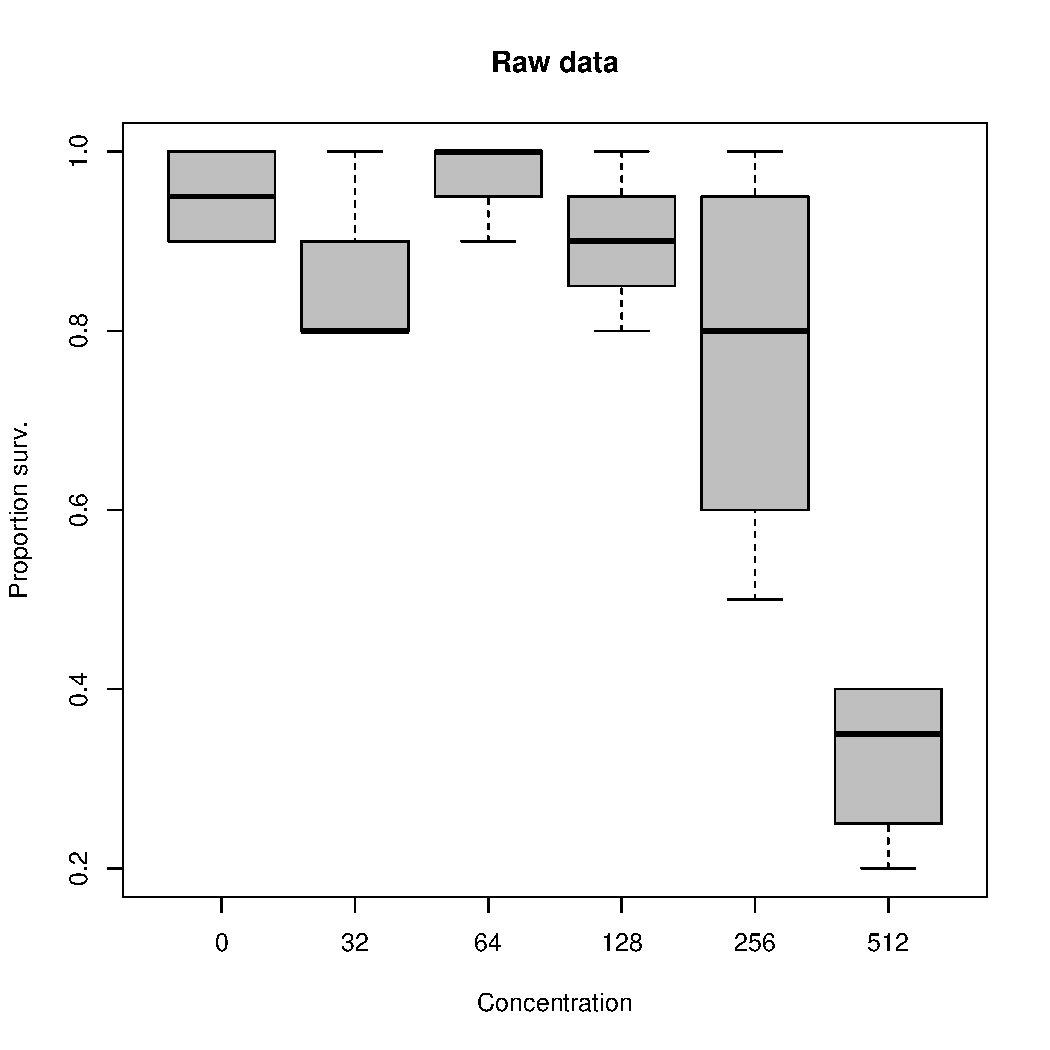
\includegraphics[width=0.5\textwidth]{figure/bin_raw_plot-1} 

\end{knitrout}
This plot indicates a strong effect at the highest concentration.


\subsubsection{Transforming data}
Next we arcsine transform the proportions:
\begin{knitrout}
\definecolor{shadecolor}{rgb}{0.969, 0.969, 0.969}\color{fgcolor}\begin{kframe}
\begin{alltt}
\hlstd{dfm}\hlopt{$}\hlstd{y_asin} \hlkwb{<-} \hlkwd{ifelse}\hlstd{(dfm}\hlopt{$}\hlstd{y} \hlopt{==} \hlnum{1}\hlstd{,}
                     \hlkwd{asin}\hlstd{(}\hlnum{1}\hlstd{)} \hlopt{-} \hlkwd{asin}\hlstd{(}\hlkwd{sqrt}\hlstd{(}\hlnum{1}\hlopt{/}\hlnum{40}\hlstd{)),}
                     \hlkwd{ifelse}\hlstd{(dfm}\hlopt{$}\hlstd{y} \hlopt{==} \hlnum{0}\hlstd{,}
                            \hlkwd{asin}\hlstd{(}\hlkwd{sqrt}\hlstd{(}\hlnum{1}\hlopt{/}\hlnum{40}\hlstd{)),}
                            \hlkwd{asin}\hlstd{(}\hlkwd{sqrt}\hlstd{(dfm}\hlopt{$}\hlstd{y))}
                            \hlstd{)}
                     \hlstd{)}
\end{alltt}
\end{kframe}
\end{knitrout}


\begin{knitrout}
\definecolor{shadecolor}{rgb}{0.969, 0.969, 0.969}\color{fgcolor}\begin{kframe}
\begin{alltt}
\hlkwd{boxplot}\hlstd{(y_asin} \hlopt{~} \hlstd{conc,} \hlkwc{data} \hlstd{= dfm,}
        \hlkwc{xlab} \hlstd{=} \hlstr{'Concentration'}\hlstd{,} \hlkwc{ylab} \hlstd{=} \hlstr{'Proportion surv.'}\hlstd{,}
        \hlkwc{main} \hlstd{=} \hlstr{'Transformed data'}\hlstd{,} \hlkwc{col} \hlstd{=} \hlstr{'grey75'}\hlstd{)}
\end{alltt}
\end{kframe}
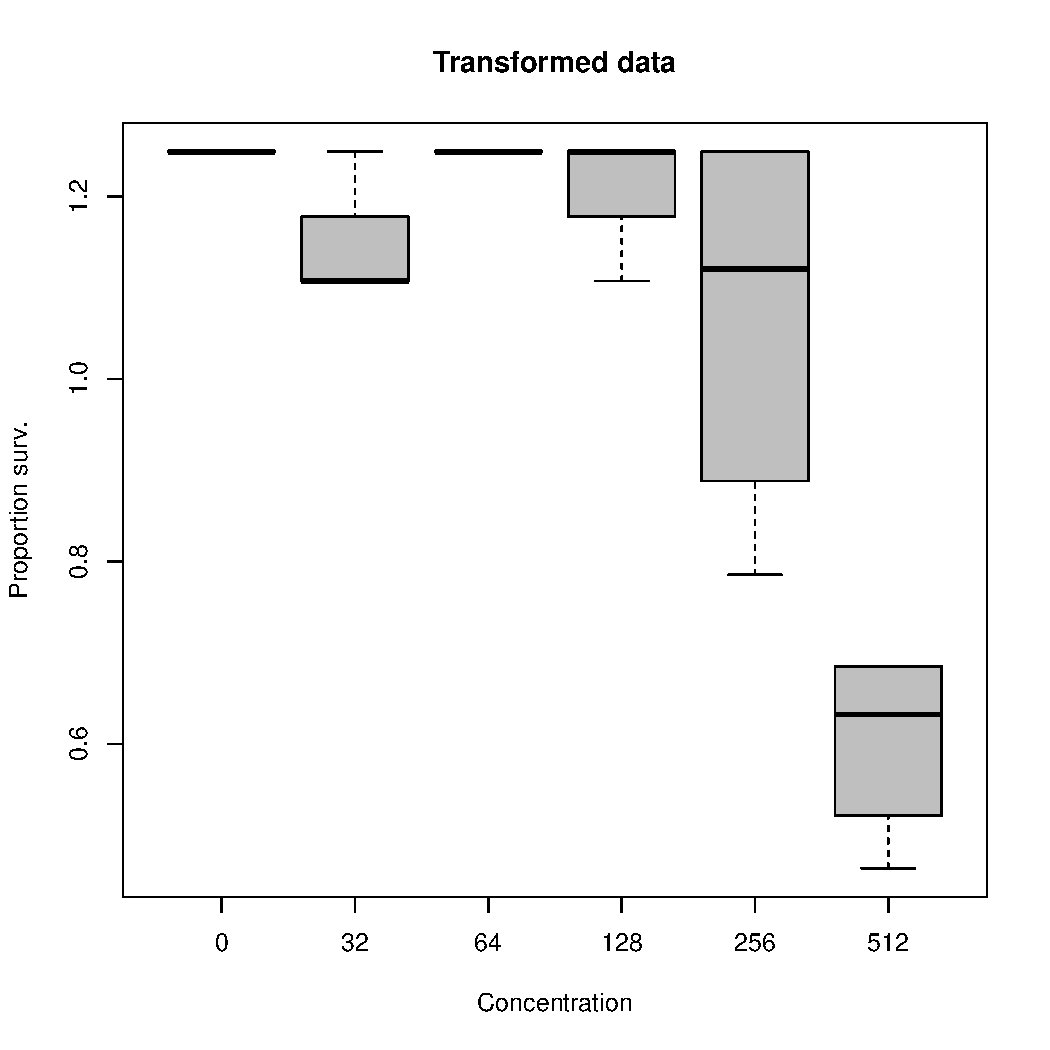
\includegraphics[width=0.5\textwidth]{figure/bin_trans_plot-1} 

\end{knitrout}

\subsubsection{Assuming a normal distribution of transformed proportions}
Like in the count data example we fit the model using \texttt{lm()}:
\begin{knitrout}
\definecolor{shadecolor}{rgb}{0.969, 0.969, 0.969}\color{fgcolor}\begin{kframe}
\begin{alltt}
\hlstd{modlm} \hlkwb{<-} \hlkwd{lm}\hlstd{(y_asin} \hlopt{~} \hlstd{conc,} \hlkwc{data} \hlstd{= dfm)}
\end{alltt}
\end{kframe}
\end{knitrout}

The summary gives the estimated parameters:
\begin{knitrout}
\definecolor{shadecolor}{rgb}{0.969, 0.969, 0.969}\color{fgcolor}\begin{kframe}
\begin{alltt}
\hlkwd{summary}\hlstd{(modlm)}
\end{alltt}
\begin{verbatim}
## 
## Call:
## lm(formula = y_asin ~ conc, data = dfm)
## 
## Residuals:
##      Min       1Q   Median       3Q      Max 
## -0.32401 -0.08149 -0.00527  0.08150  0.30261 
## 
## Coefficients:
##             Estimate Std. Error t value Pr(>|t|)    
## (Intercept)  1.33053    0.07693  17.295 1.16e-12 ***
## conc32      -0.14717    0.10880  -1.353   0.1929    
## conc64       0.04074    0.10880   0.374   0.7124    
## conc128     -0.07622    0.10880  -0.701   0.4925    
## conc256     -0.22113    0.10880  -2.032   0.0571 .  
## conc512     -0.72735    0.10880  -6.685 2.86e-06 ***
## ---
## Signif. codes:  0 '***' 0.001 '**' 0.01 '*' 0.05 '.' 0.1 ' ' 1
## 
## Residual standard error: 0.1539 on 18 degrees of freedom
## Multiple R-squared:  0.7871,	Adjusted R-squared:  0.7279 
## F-statistic: 13.31 on 5 and 18 DF,  p-value: 1.612e-05
\end{verbatim}
\end{kframe}
\end{knitrout}

The F-test suggests a treatment related effect:
\begin{knitrout}
\definecolor{shadecolor}{rgb}{0.969, 0.969, 0.969}\color{fgcolor}\begin{kframe}
\begin{alltt}
\hlkwd{drop1}\hlstd{(modlm,} \hlkwc{test} \hlstd{=} \hlstr{'F'}\hlstd{)}
\end{alltt}
\begin{verbatim}
## Single term deletions
## 
## Model:
## y_asin ~ conc
##        Df Sum of Sq     RSS     AIC F value    Pr(>F)    
## <none>              0.42613 -84.746                      
## conc    5    1.5753 2.00142 -57.621  13.308 1.612e-05 ***
## ---
## Signif. codes:  0 '***' 0.001 '**' 0.01 '*' 0.05 '.' 0.1 ' ' 1
\end{verbatim}
\end{kframe}
\end{knitrout}

And the LOEC is at the highest concentration:
\begin{knitrout}
\definecolor{shadecolor}{rgb}{0.969, 0.969, 0.969}\color{fgcolor}\begin{kframe}
\begin{alltt}
\hlkwd{summary}\hlstd{(}\hlkwd{glht}\hlstd{(modlm,} \hlkwc{linfct} \hlstd{=} \hlkwd{mcp}\hlstd{(}\hlkwc{conc} \hlstd{=} \hlstr{'Dunnett'}\hlstd{),} \hlkwc{alternative} \hlstd{=} \hlstr{'less'}\hlstd{))}
\end{alltt}
\begin{verbatim}
## 
## 	 Simultaneous Tests for General Linear Hypotheses
## 
## Multiple Comparisons of Means: Dunnett Contrasts
## 
## 
## Fit: lm(formula = y_asin ~ conc, data = dfm)
## 
## Linear Hypotheses:
##              Estimate Std. Error t value Pr(<t)    
## 32 - 0 >= 0  -0.14717    0.10880  -1.353 0.2785    
## 64 - 0 >= 0   0.04074    0.10880   0.374 0.9202    
## 128 - 0 >= 0 -0.07622    0.10880  -0.701 0.5577    
## 256 - 0 >= 0 -0.22113    0.10880  -2.032 0.0986 .  
## 512 - 0 >= 0 -0.72735    0.10880  -6.685 <0.001 ***
## ---
## Signif. codes:  0 '***' 0.001 '**' 0.01 '*' 0.05 '.' 0.1 ' ' 1
## (Adjusted p values reported -- single-step method)
\end{verbatim}
\end{kframe}
\end{knitrout}


\subsubsection{Assuming a binomial distribution}
The binomial model with a logit link between predictors and response can be fitted using the \texttt{glm()} function:
\begin{knitrout}
\definecolor{shadecolor}{rgb}{0.969, 0.969, 0.969}\color{fgcolor}\begin{kframe}
\begin{alltt}
\hlstd{modglm} \hlkwb{<-} \hlkwd{glm}\hlstd{(y} \hlopt{~} \hlstd{conc ,} \hlkwc{data} \hlstd{= dfm,} \hlkwc{family} \hlstd{=} \hlkwd{binomial}\hlstd{(}\hlkwc{link} \hlstd{=} \hlstr{'logit'}\hlstd{),}
              \hlkwc{weights} \hlstd{=} \hlkwd{rep}\hlstd{(}\hlnum{10}\hlstd{,} \hlkwd{nrow}\hlstd{(dfm)))}
\end{alltt}
\end{kframe}
\end{knitrout}

Here the weights arguments, indicates how many fish where exposed in each treatment (=10).

The summary gives the estimated parameters:
\begin{knitrout}
\definecolor{shadecolor}{rgb}{0.969, 0.969, 0.969}\color{fgcolor}\begin{kframe}
\begin{alltt}
\hlkwd{summary}\hlstd{(modglm)}
\end{alltt}
\begin{verbatim}
## 
## Call:
## glm(formula = y ~ conc, family = binomial(link = "logit"), data = dfm, 
##     weights = rep(10, nrow(dfm)))
## 
## Deviance Residuals: 
##     Min       1Q   Median       3Q      Max  
## -1.8980  -0.5723   0.0000   0.7869   2.2578  
## 
## Coefficients:
##             Estimate Std. Error z value Pr(>|z|)    
## (Intercept)   2.9444     0.7255   4.059 4.94e-05 ***
## conc32       -1.2098     0.8499  -1.423   0.1546    
## conc64        0.7191     1.2458   0.577   0.5638    
## conc128      -0.7472     0.8967  -0.833   0.4047    
## conc256      -1.7077     0.8183  -2.087   0.0369 *  
## conc512      -3.6753     0.8002  -4.593 4.37e-06 ***
## ---
## Signif. codes:  0 '***' 0.001 '**' 0.01 '*' 0.05 '.' 0.1 ' ' 1
## 
## (Dispersion parameter for binomial family taken to be 1)
## 
##     Null deviance: 88.672  on 23  degrees of freedom
## Residual deviance: 23.889  on 18  degrees of freedom
## AIC: 72.862
## 
## Number of Fisher Scoring iterations: 5
\end{verbatim}
\end{kframe}
\end{knitrout}

To perform a LR-test we can used the \texttt{drop1()} function:
\begin{knitrout}
\definecolor{shadecolor}{rgb}{0.969, 0.969, 0.969}\color{fgcolor}\begin{kframe}
\begin{alltt}
\hlkwd{drop1}\hlstd{(modglm,} \hlkwc{test} \hlstd{=} \hlstr{'Chisq'}\hlstd{)}
\end{alltt}
\begin{verbatim}
## Single term deletions
## 
## Model:
## y ~ conc
##        Df Deviance     AIC    LRT  Pr(>Chi)    
## <none>      23.889  72.862                     
## conc    5   88.672 127.645 64.783 1.243e-12 ***
## ---
## Signif. codes:  0 '***' 0.001 '**' 0.01 '*' 0.05 '.' 0.1 ' ' 1
\end{verbatim}
\end{kframe}
\end{knitrout}

Also with the binomial model the LOEC is at the highest concentration:
\begin{knitrout}
\definecolor{shadecolor}{rgb}{0.969, 0.969, 0.969}\color{fgcolor}\begin{kframe}
\begin{alltt}
\hlkwd{summary}\hlstd{(}\hlkwd{glht}\hlstd{(modglm,} \hlkwc{linfct} \hlstd{=} \hlkwd{mcp}\hlstd{(}\hlkwc{conc} \hlstd{=} \hlstr{'Dunnett'}\hlstd{),} \hlkwc{alternative} \hlstd{=} \hlstr{'less'}\hlstd{))}
\end{alltt}
\begin{verbatim}
## 
## 	 Simultaneous Tests for General Linear Hypotheses
## 
## Multiple Comparisons of Means: Dunnett Contrasts
## 
## 
## Fit: glm(formula = y ~ conc, family = binomial(link = "logit"), data = dfm, 
##     weights = rep(10, nrow(dfm)))
## 
## Linear Hypotheses:
##              Estimate Std. Error z value Pr(<z)    
## 32 - 0 >= 0   -1.2098     0.8499  -1.423  0.203    
## 64 - 0 >= 0    0.7191     1.2458   0.577  0.923    
## 128 - 0 >= 0  -0.7472     0.8967  -0.833  0.432    
## 256 - 0 >= 0  -1.7077     0.8183  -2.087  0.059 .  
## 512 - 0 >= 0  -3.6753     0.8002  -4.593 <0.001 ***
## ---
## Signif. codes:  0 '***' 0.001 '**' 0.01 '*' 0.05 '.' 0.1 ' ' 1
## (Adjusted p values reported -- single-step method)
\end{verbatim}
\end{kframe}
\end{knitrout}







\bibliography{references}
\bibliographystyle{apalike}


\end{document} 
